%!TEX program = xelatex
\documentclass[10pt]{article}
\usepackage{amssymb}
\usepackage{amsmath}
\usepackage{mathrsfs}
\usepackage{titlesec}
\usepackage{xcolor}
%\usepackage[shortlabels]{enumitem}
\usepackage{enumerate}
\usepackage{bm}
\usepackage{tikz}
\usepackage{listings}
\usetikzlibrary{arrows}
\usepackage{subfigure}
\usepackage{graphicx,booktabs,multirow}
\usepackage[a4paper]{geometry}
\usepackage{upquote}
\usepackage{float}
\usepackage{pdfpages}

\usepackage[colorlinks,linkcolor=blue]{hyperref}
\usepackage{mdframed}

\iffalse
\usepackage{lastpage}
\usepackage{fancyhdr}
\fancyfoot[C]{Page \thepage\ of \pageref{LastPage}}
% Uncomment to remove the header rule
\renewcommand{\headrulewidth}{0pt} 
\pagestyle{fancy}
\fi

\geometry{verbose,tmargin=2cm,bmargin=2cm,lmargin=2cm,rmargin=2cm}
\geometry{verbose,tmargin=2cm,bmargin=2cm,lmargin=2cm,rmargin=2cm}
\lstset{language=Matlab}
\lstset{breaklines}

\input defs.tex

\newenvironment{solution}
    { \begin{mdframed}[backgroundcolor=gray!10] \textcolor{cyan}{\textbf{Solution}} \\}
    {  \end{mdframed}}

\newtheorem{proposition}{Proposition}
\newtheorem{remark}{Remark}

\titleformat*{\section}{\centering\LARGE\scshape}
\renewcommand{\thesection}{\Roman{section}}
\lstset{language=Matlab,tabsize=4,frame=shadowbox,basicstyle=\footnotesize,
keywordstyle=\color{blue!90}\bfseries,breaklines=true,commentstyle=\color[RGB]{50,50,50},stringstyle=\ttfamily,numbers=left,numberstyle=\tiny,
  numberstyle={\color[RGB]{192,92,92}\tiny},backgroundcolor=\color[RGB]{245,245,244},inputpath=code}

\begin{document}

%\title{CS150: Database and Data Mining \\%
%	Final Exam}
%\maketitle


\newpage
\section{SQL \textbf{[10 points]}}
Suppose that you are running a pet store. You want to manage the information of your customers and dogs of your store.
You begin with several tables as follow. For each question, there may be one, or more than one correct answer.
\begin{verbatim}
CREATE TABLE users (
userid INTEGER,
name STRING,
age INTEGER,
PRIMARY KEY (userid)
);
\end{verbatim}

\begin{verbatim}
CREATE TABLE dogs (
dogid INTEGER,
owner INTEGER,
name STRING,
breed STRING,
age INTEGER,
PRIMARY KEY (dogid),
FOREIGN KEY (owner) REFERENCES users
);
\end{verbatim}

\begin{enumerate}
	\item \textbf{[3 points]}
	      Suppose you need to know the number of dog breeds of all your dogs, select the correct SQL query:\\
	      A.
	      \begin{lstlisting} 
		SELECT COUNT(*) 
		FROM dogs;
	\end{lstlisting}
	      B.
	      \begin{lstlisting}
		SELECT * 
		FROM dogs 
		GROUP BY breed;
	\end{lstlisting}
	      C.
	      \begin{lstlisting}
		SELECT COUNT(breed) 
		FROM dogs;
	\end{lstlisting}
	      D.
	      \begin{lstlisting}
		SELECT COUNT(DISTINCT breed) 
		FROM dogs;
	\end{lstlisting}
	      E.
	      \begin{lstlisting}
		SELECT * 
		FROM dogs;
	\end{lstlisting}
	      % Answer: d

	\item \textbf{[3 points]}
	      Which query	should you issue to find the userid of the user with the most dogs along with the number of dogs the user owns?
	      The query should return only one row in the case where there are multiple users	with the same number of dogs. \\
	      A.
	      \begin{lstlisting}
        SELECT userid, COUNT(*) as cnt
        FROM dogs, users
        WHERE userid = dogid
        ORDER BY cnt DESC
        LIMIT 1;
    \end{lstlisting}
	      B.
	      \begin{lstlisting}
        SELECT userid, MAX(dogid) as max
        FROM dogs,users
        WHERE userid = owner
        GROUP BY dogid, userid
        ORDER BY max DESC
        LIMIT 1;
    \end{lstlisting}
	      C.
	      \begin{lstlisting}
        SELECT userid, COUNT(*) as cnt
        FROM dogs INNER JOIN users ON userid = owner
        GROUP BY userid
        ORDER BY cnt DESC
        LIMIT 1;
    \end{lstlisting}
	      D.
	      \begin{lstlisting}
        SELECT userid, COUNT(*) as cnt
        FROM dogs LEFT OUTER JOIN users ON userid = dogid
        GROUP BY userid;
    \end{lstlisting}
	      E.
	      \begin{lstlisting}
        SELECT userid, COUNT(*) as cnt
        FROM dogs,users
        WHERE userid = owner
        GROUP BY userid
        ORDER BY cnt DESC
        LIMIT 1;
    \end{lstlisting}
	      %   Answer: c e

	\item \textbf{[4 points]}
	      Please give the non-nested query that finds the most popular breed
	      (in other words, the breed of dogs chosen by the most owners.) along with the number of dogs.

	      %   Answer: T
	      %    e.g.
	      %   \begin{verbatim}
	      %   select breed, count(*) as cnt
	      %  from dogs inner join users on userif = owner
	      % group by breed
	      % ordered by cnt
	      % limit 1;
	      % \end{verbatim}

\end{enumerate}
\textbf{Your answer:}
%	      \newpage\phantom{blabla}



\newpage
\section{Disk, Buffers and Files \textbf{[10 points]}}
\begin{enumerate}
	\item \textbf{[4 points]}
	      Consider the following relation:
	      \begin{verbatim}
CREATE TABLE products (
	id INTEGER, -- cannot be NULL
	stock INTEGER, -- NOT NULL
	price INTEGER, -- NOT NULL
	name VARCHAR(10), -- NOT NULL
	category CHAR(6), -- NOT NULL
	serial_number CHAR(20), -- may be NULL
	PRIMARY KEY (id)
);
\end{verbatim}
	      A field of type CHAR(n) consists of exactly n characters, while a
	      field of type VARCHAR(n) consists of at most n characters (assume
	      that a field of VARCHAR(n) takes up at most n bytes). Assume that
	      record headers take up 8 bytes, and integers are 4 bytes long. Note
	      that columns in a primary key cannot be NULL. Which of the following, if any, are a possible size,
	      in bytes, for some record of the products relation, assuming a variable-length
	      representation with a record header? There may be one, or more
	      than one correct answer. \\
	      A. 18\\
	      B. 27\\
	      C. 38\\
	      D. 45\\
	      E. 48\\
	      F. 55\\
	      %\\
	      %Solution:B,E,F (26-36, 46-56)\\
	      %\\
	      \\

	\item \textbf{[6 points]}
	      In the following two questions, assume that we are using fixed-length
	      records, and each record is 64 bytes long. Assume that the page header
	      is empty, except for a bitmap when necessary, which is as small as
	      possible, rounded up to the nearest byte.
	      \begin{itemize}
		      \item[(a)] \textbf{[3 points]} How many records can fit on a 1 KB page, assuming we
		            use a packed page layout?
		            %Solution: 1024/64=16\\
		      \item[(b)] \textbf{[3 points]} How many records can fit on a 1 KB page, assuming we
		            use an unpacked page layout?
		            %Solution: 15, because bitmap needs 15bits which is close to 2byte
	      \end{itemize}

\end{enumerate}
\textbf{Your answer:}
%     \newpage\phantom{blabla}



\newpage
\section{File Organization \textbf{[12 points]}}
In I/O (Input/Output) cost model for analysis, we define: \\
\textbf{B}: the number of data blocks in the file;\\
\textbf{R}: the number of records per block;\\
\textbf{D}: average time to read/write one disk block.\\
Please answer the following questions:
\begin{enumerate}
	\item \textbf{[4 points]}
	      Please compare the I/O cost of range search in heap file and sorted file? Correct answer without proper explanation will earn no scores.  \\
	\item \textbf{[4 points]}
	      Please compare the I/O cost of deletion of a single record in heap file and sorted file? Correct answer without proper explanation will earn no scores.  \\
	\item \textbf{[4 points]}
	      Is there any type of file organization to reduce the I/O cost of deletion? If yes, show the type and its I/O cost.
\end{enumerate}
\textbf{Your answer:}
%      \newpage\phantom{blabla}



\newpage
\section{Indexes and B+ Trees \textbf{[12 points]}}
\begin{enumerate}

	\item \textbf{[2 points]}
	      For the B+ trees below, determine which of the trees are valid B+ trees, and fill in its corresponding box on the answer sheet.
	      Assume that there were no deletes. Note, we follow the right branch when the split key equals the search key.
	      There may be zero, one, or more than one correct answer.

	      A.

	      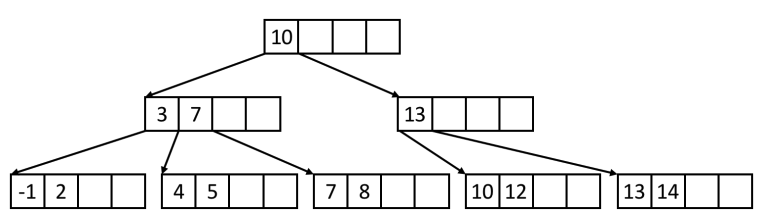
\includegraphics[scale=0.4]{3.png}

	      B.

	      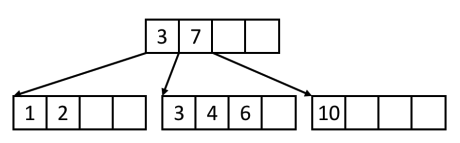
\includegraphics[scale=0.4]{1.png}

	      C.

	      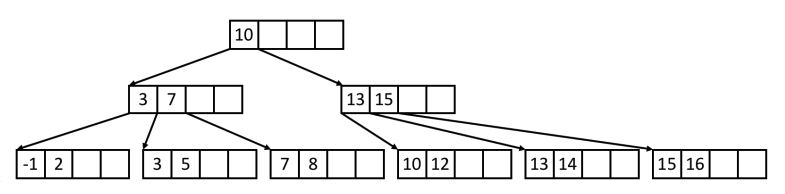
\includegraphics[scale=0.4]{4.png}

	      D.

	      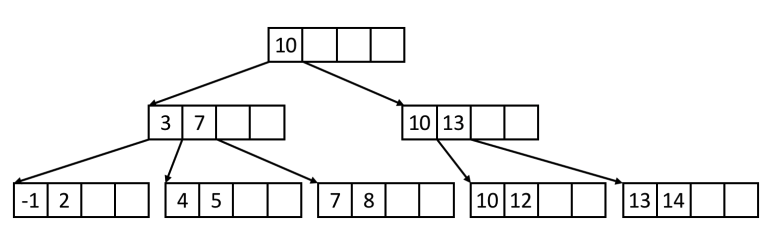
\includegraphics[scale=0.4]{2.png}
	      %Answer: c
	      \\

	\item \textbf{[5 points]}
	      What is the minimum number of inserts we can do that will change the height of the following tree?
	      \begin{center}
		      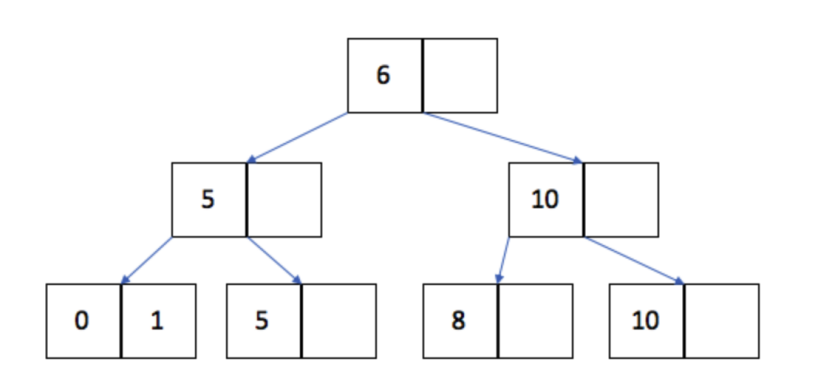
\includegraphics[scale=0.3]{5.png}
	      \end{center}
	      %Answer: 4. One possible pattern is 2,3,4,4.1.

	\item \textbf{[5 points]}
	      What is the resulting B+ tree after bulk loading the keys: $3, 8, 5, 19, 20, 11, 7$?
	      Assume we are building an order $d=1$ index with a minimum leaf node fill factor of $2/3$.
	      %Answer: 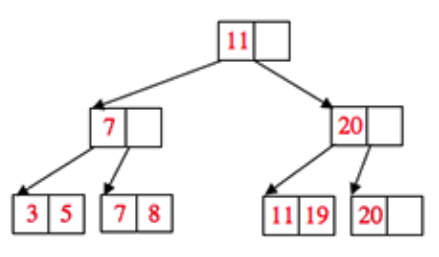
\includegraphics[scale=0.4]{6.png}

\end{enumerate}
\textbf{Your answer:}
\newpage\phantom{blabla}



\newpage
\section{Buffer Management \textbf{[12 points]}}
For any question that asks which pages are in the buffer pool at some point in time, please list the pages in alphabetical order.
Assume we have 4 empty buffer frames and the following access pattern, in which pages are immediately unpinned: \\
A, C, D, F, D, C, B, C, A, E, C, D \\

\begin{enumerate}
	\item \textbf{[4 points]}
	      Which pages are in the buffer pool at the end if we use MRU policy?   \\

	      %   Answer:  CDEF

	\item \textbf{[4 points]}
	      Which pages are in the buffer pool at the end if we use Clock policy? (reference bit is set when a page is loaded in buffer)  \\
	      %  Answer: ACDE

	\item \textbf{[4 points]}
	      Assume we have 4 empty buffer frames and the following access pattern, in which pages are immediately unpinned: \\
	      A, B, C, D, E, A, B, C, D, E, A, B, C, D, E \\
	      How many cache hits will occur if we use LRU policy?
	      %  Answer: 0

\end{enumerate}
\textbf{Your answer:}
%  \newpage\phantom{blabla}



\newpage
\section{Relational Algebra \textbf{[10 points]}}
For the following relational algebra questions, please use the schema
defined below.\\

Students(sid, sname, year) \\

Companies(cid, cname, valuation) \\

Recruitment(sid, cid, position, salary, status) \\
\\
For each question, indicate which of the expressions gives the desired
output. Note that the following table abbreviations are being used:
Students $\rightarrow$ S, Companies $\rightarrow$ C, Recruitment
$\rightarrow$ R. Also note that some of the expressions are invalid,
in which case they should definitely not be marked in your answer.

\begin{enumerate}
	\item \textbf{[3 points]} Find the names of all students who have received at
	      least one recruitment offer. Note that if a student has received an
	      offer, the status field in the Recruitment table will be the text
	      \textquotedblleft offer\textquotedblright . Mark all that apply.\\
	      A. $\pi_{\text{sname }}\left(\sigma_{\text{status }="\text{offer}"}(S\bowtie R)\right)$\\
	      B. $\pi_{\text{sname }}\left(S\bowtie\left(\sigma_{\text{status }="\text{offer}"}(R)\right)\right)$\\
	      C. $\sigma_{\text{status }="\text{\text{offer}"}}\left(\left(\pi_{\text{sname }}(S)\right)\bowtie R\right)$\\
	      D. $\pi_{\text{sname }}\left(\sigma_{\text{status }="\text{offer}"}\left(S\bowtie\left(\pi_{sid}(R)\right)\right)\right)$\\
	      %Solution: A,B\\
	      \\
	\item \textbf{[3 points]} Find the names of all students who have not received
	      an offer from any company. Mark all that apply.\\
	      A. $\pi_{\text{sname }}\left(\left(\sigma_{\text{status="of fer}^{\prime\prime}}\left(\pi_{\text{sid }}(S)-\pi_{\text{sid }}(R)\right)\right)\bowtie S\right)$\\
	      B. $\pi_{\text{sname }}\left(\left(\pi_{\text{sid }}(S)-\pi_{\text{sid }}\left(\sigma_{\text{status="offer}^{\prime\prime}}(R)\right)\right)\bowtie S\right)$\\
	      C. $\pi_{\text{sname }}(S)-\pi_{\text{sname }}\left(\sigma_{\text{status }=\text{ "offer}^{\prime\prime}}(R\bowtie S)\right)$\\
	      D. $\sigma_{\text{status }=\text{ "offer}^{\prime\prime}}\left(\left(\pi_{\text{sname }}\left(\pi_{\text{sid }}(S)-\pi_{\text{sid }}(R)\right)\right)\bowtie S\right)$\\
	      %Solution: B\\
	      \\
	\item \textbf{[4 points]} For every record in Recruitment, output the name of
	      the student, name of the company he/she is being recruited for, and
	      the position the student is being recruited for. Mark all that apply.\\
	      A. $\left(\pi_{\text{sname }}(S)\right)\bowtie\left(\pi_{\text{cname }}(C)\right)\bowtie\left(\pi_{\text{position }}(R)\right)$\\
	      B. $\pi_{\text{sname, cname, position }}(S\bowtie C\bowtie R)$\\
	      C. $\pi_{\text{sname, cname, position }}\left(\left(\pi_{\text{sid },\text{ sname }}(S)\right)\bowtie\left(\pi_{\text{cid, cname }}(C)\right)\bowtie\left(\pi_{\text{position }}(R)\right)\right)$\\
	      D. $\pi_{\text{sname, cname, position }}\left(S\bowtie C\bowtie\left(\pi_{\text{sid, cid, position }}(R)\right)\right)$\\
	      %Solution: B,D\\
\end{enumerate}
\textbf{Your answer:}
%    \newpage\phantom{blabla}


\newpage
\section{Sorting and Hashing \textbf{[12 points]}}
For this question, consider a table of Products (P), and assume:
\begin{itemize}
	\item $[P] = 2000$ pages
	\item $p_c = 100$ tuples/page
	\item $B = 40$ pages of buffer
	\item In all parts, we’ll use QuickSort for our internal sort algorithm.
	\item Include the cost of the initial scan and cost of writing output in your I/O calculations.
\end{itemize}

\begin{enumerate}
	\item \textbf{[4 points]}
	      First, let’s sort our table of Products (P) using the external algorithm we learned in lecture.
	      \begin{itemize}
		      \item[(a)] How many passes are needed to sort this file?
		      \item[(b)] What is the I/O cost (in pages) of sorting this file?
	      \end{itemize}
	\item \textbf{[4 points]}
	      What is the largest file size (in pages) that we can sort in 2 passes?\\
	\item \textbf{[4 points]}
	      Suppose I want to eliminate duplicates from our (unsorted) table of Products,
	      using external hashing. Write down the letters of true statements.
	      \begin{itemize}
		      \item[A.] De-duplicating the file using hashing can have a higher IO cost than sorting the file (without deduplicating).
		      \item[B.] De-duplicating the file using hashing can have a lower IO cost than sorting the file (without deduplicating).
	      \end{itemize}
\end{enumerate}
\textbf{Your answer:}
%      \newpage\phantom{blabla}



\newpage
\section{Iterations and Joins \textbf{[12 points]}}
There are two tables: Candies and Stores. \\

Candies(cid int, cname text, manufacturer text) \\

Stores(sid int, sname text, cid int) \\
\\
You want to see which stores carry your favorite candies, but you are unsure of which join
algorithm you should utilize to perform the query below.
\begin{verbatim}
SELECT C.cid, COUNT(*)
FROM Candies C, Stores S
WHERE C.cid = S.cid
GROUP BY C.cid;
\end{verbatim}

\noindent
We have 100 pages of Candies and 60 pages of Stores. The Candies table has 5 records per
page, and the Stores table has 10 records per page. Be sure to choose the inner and outer relations such that you minimize the I/O cost. You have 25 buffer pages at your disposal.


\begin{enumerate}
	\item \textbf{[3 points]}
	      What is the I/O cost of a block nested loops join between Candies and Stores? \\
	\item \textbf{[3 points]}
	      What is the I/O cost of an index nested loops join between Candies and Stores?
	      (There is an index on Stores.cid, and it takes an average of 3 I/O's to find a matching tuple.) \\
	\item \textbf{[3 points]}
	      What is the I/O cost of a sort-merge join between Candies and Stores? \\
	\item \textbf{[3 points]}
	      What is the I/O cost of a grace hash join between Candies and Stores?
	      (Assume we have hash functions that can partition the data evenly.)
\end{enumerate}
\textbf{Your answer:}
%  \newpage\phantom{blabla}




\newpage
\section{Query Optimization \textbf{[10 points]}}
%\subsection{Selectivity Estimation}
Consider two relations Cat(age, weight, price) and Pocket(money), with 150 tuples and 100 tuples respectively.
We have an index on Cat.age with 15 unique integer values uniformly distributed in the range [1, 15],
an index on Cat.weight with 30 unique float values uniformly distributed in the range [2001, 5000],
an index on Cat.price with 10 unique integer values uniformly distributed in the range [11, 20],
and an index on Pocket.money with 15 unique integer values uniformly distributed in the range [11, 25]. \\
%We do not have an index on Cat.price.\\
Use selectivity estimation to estimate the number of tuples produced by the following queries.
\begin{enumerate}
	\item \textbf{[3 point]} SELECT * FROM Cat\\
	\item \textbf{[3 points]} SELECT * FROM Cat WHERE age $\geq$ 10\\
	\item \textbf{[4 points]} SELECT * FROM Cat WHERE age $\textless$ 5 AND weight $\leq$ 3000\\
	      %	\item[(d)] \textbf{[2 points]} SELECT * FROM Cat WHERE age $\textgreater$ 10 OR price $\geq$ 15\\
	      %	\item[(e)] \textbf{[3 points]} SELECT * FROM Cat, Pocket WHERE Cat.price = Pocket.money\\
\end{enumerate}
\textbf{Your answer:}
%   \newpage\phantom{blabla}

\end{document}

